% This text is proprietary.
% It's a part of presentation made by myself.
% It may not used commercial.
% The noncommercial use such as private and study is free
% Sep. 2005
% Author: Sascha Frank
% University Freiburg
% www.informatik.uni-freiburg.de/~frank/


\documentclass{beamer}
%% \usetheme{Warsaw}

\usepackage{color}
\usepackage{booktabs}
\usepackage{tikz}
\usepackage{graphicx}
\usepackage{caption}
\usepackage{subcaption}
\setbeamertemplate{navigation symbols}{}
\setbeamerfont{page number in head/foot}{size=\normalsize}
\setbeamertemplate{footline}[frame number]
\usetikzlibrary{positioning}
\AtBeginSection{\frame{\sectionpage}}
%% \AtBeginSubsection{\frame{\subsectionpage}}

\newcommand*\nodestatecolor{green}
\newcommand*\scalefilter{1}
\newcommand*\initialstatetext{Previous State}
\newcommand*\initialstatecolor{yellow}

\tikzstyle{input}=[draw,fill=yellow,minimum width=2.6cm,thin]
\tikzstyle{method}=[draw,fill=pink,minimum width=1.8cm]
\tikzstyle{arr}=[-latex,ultra thick]
\tikzstyle{dummy}=[minimum width=2.6cm]


\title{Absolute scale velocity determination
combining visual and inertial
measurements for micro aerial
vehicles}
\subtitle{}
\date{June 24, 2015}
\author{Jacques Kaiser}
\institute{INRIA}

\begin{document}

\maketitle

\section{Sensor fusion}

\begin{frame}{Micro aerial vehicles}
\includegraphics<1>[width=0.6\textwidth]{images/drone.png}
\includegraphics<2>[width=0.6\textwidth]{images/droneState.png}
\includegraphics<3->[width=0.6\textwidth]{images/dronePointState.png}

\onslide<4->

%drone is a rigid body - you can reduce it to a point
\begin{columns}[T] % contents are top vertically aligned
\column{.5\textwidth}
\centering
A basic state vector:
\[
X =
\left[
\begin{array}{c}
r \\ \dot{r}\\ q
\end{array}
\right]
\]

\column{.5\textwidth}
        \begin{itemize}
        \item $r$ position;
        \item $\dot{r}$ velocity;
        \item $q$ orientation.
        \end{itemize}
\end{columns}

\onslide<5->
\textbf{The goal of sensor fusion is to recover the state $X$}

\end{frame}

\subsection{Filter based fusion}

\begin{frame}{Visual-inertial sensor fusion}

{\centering
\textbf{Filter based method}

\only<2->{\renewcommand*\nodestatecolor{yellow}}
\only<2->{\renewcommand*\scalefilter{0.7}}
\only<4->{\renewcommand*\initialstatecolor{blue!60}}
\only<4->{\renewcommand*\initialstatetext{Initial State}}

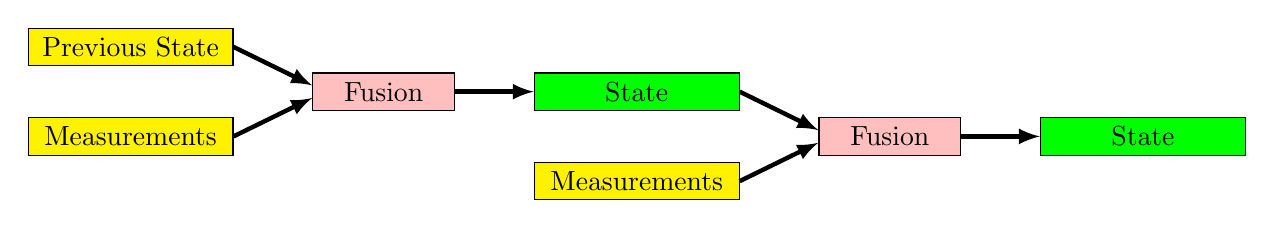
\begin{tikzpicture}[scale=\scalefilter, every node/.style={transform shape}]

\node (A) [input, fill=\initialstatecolor] {\initialstatetext};
\node (dummy1) [dummy, below=2mm of A] {};
\node (C) [input,below=2mm of dummy1] {Measurements};
\node (D) [method,right=of dummy1] {Fusion};
\node (E) [input, right=of D, fill=\nodestatecolor] {State};

\node<2-> (dummy2) [dummy, below=2mm of E] {};
\node<2-> (F) [input, below=2mm of dummy2] {Measurements};


\node<3-> (G) [method, right=of dummy2] {Fusion};
\node<3-> (H) [input, right=of G, fill=green] {State};

\draw[arr] (A.east) -- (D.175);
\draw[arr] (C.east) -- (D.185);
\draw[arr] (D.east) -- (E.west);
\draw<3->[arr] (E.east) -- (G.175);
\draw<3->[arr] (F.east) -- (G.185);
\draw<3->[arr] (G.east) -- (H.west);

\end{tikzpicture}
}

\onslide<4->
How to recover the \textbf{initial state}?

\onslide<5->
We need a \textbf{deterministic solution}

\vspace{0.5cm}
{\centering
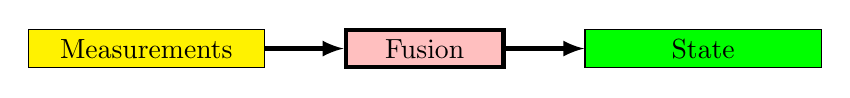
\begin{tikzpicture}
\tikzstyle{input}=[draw,fill=yellow,minimum width=3cm,thin]
\tikzstyle{method}=[draw,fill=pink,minimum width=2cm]
\tikzstyle{every path}=[-latex,ultra thick]
\node (C) [input] {Measurements};
\node (D) [method,right=of C] {Fusion};
\node (E) [input, right=of D, fill=green] {State};



\draw (C.east) -- (D.west);
\draw (D.east) -- (E.west);
\end{tikzpicture}
}

\end{frame}

\subsection{Deterministic solution}

\begin{frame}{Deterministic solutions in Computer Vision}

\begin{figure}
\centering
\includegraphics[width=0.5\textwidth]{images/directMethod.png}
\end{figure}

\onslide<2->
\begin{itemize}
\item 8-point algorithm;
\item sparse model-based image alignment;
\item ...
\end{itemize}

\onslide<3->

But the relative translation and distance to features are recovered only \textbf{up to scale}

% Camera is an angle sensor
\end{frame}


{ % all template changes are local to this group.
    \setbeamertemplate{navigation symbols}{}
    \begin{frame}[plain]{Absolute scale from visual measurements}
      How big is this building?
      \vspace{-2em}\begin{center}\includegraphics[width=\textwidth]{images/buildingDetour.png}\end{center}
     \end{frame}
}
{ % all template changes are local to this group.
    \setbeamertemplate{navigation symbols}{}
    \begin{frame}[plain]{Absolute scale from visual measurements}
      \vspace{1.1em}
      \vspace{-2em}\begin{center}\includegraphics[width=\textwidth]{images/buildingScale.jpg}\end{center}
     \end{frame}
}


%% \begin{frame}{Absolute scale from visual measurements}
%%   How big is this building?
%%   \vspace{-2em}\begin{center}\includegraphics[width=\textwidth]{images/buildingDetour.png}\end{center}

%% \end{frame}

%% % we can tell the central door is bigger than the people
%% % but now way to determine physical quantities: how big, how far, how fast is the camera moving,..
%% % Even provided with many images
%% %

%% \begin{frame}{Absolute scale from visual measurements}
%%   \vspace{-2em}\begin{center}\includegraphics[width=\textwidth]{images/buildingScale.jpg}\end{center}
%% \end{frame}
%% % We need to known a physical quantity to set the absolute scale
%% % That's how drones are initialized..


\begin{frame}{Methods to recover the absolute scale}


  \includegraphics[width=0.45\textwidth]{images/referenceInEnv.png}~
  \includegraphics<2->[width=0.45\textwidth]{images/altitudeSensor.png}

  \begin{columns}[T] % contents are top vertically aligned
    \column<3->{.46\textwidth}
    \centering
    Not suited to unknown environments

    \column<3->{.5\textwidth}
    \centering
    Unprecise, works only in hover
\end{columns}

\end{frame}

% so far we only considered visual measurements
% the IMU provides physical quantity (m/s^2 and rad/s)
\begin{frame}{Inertial Measurement Unit (IMU)}

The IMU consists of two sensors providing \textbf{physical quantities}:
\begin{itemize}
\item Accelerometer: linear acceleration ($m/s^2$);
\item Gyroscope: angular velocity ($rad/s$).
\end{itemize}

\end{frame}

\begin{frame}{Title}
absolute scale velocity determination combining visual and inertial measurements for micro aerial vehicles
\end{frame}
% \begin{frame}{Dead reckoning}
% Provided only with inertial measurements, we are subject to drift.

% %bias ?
% \end{frame}



% So far, knowledge of previous state was required. Now we have a Closed-form solution that only relies on measurements over a short interval of time
\begin{frame}{The closed-form solution - 2014}

Deterministic solution


Input:
\begin{itemize}
\item Matching point-features over a time interval; \hfill \onslide<2->{\textcolor{red}{camera}}
\item Linear acceleration; \hfill \onslide<2->{\textcolor{blue}{IMU}}
\item Angular velocity; \hfill \onslide<2->{\textcolor{blue}{IMU}}
\item External Camera IMU transformation. \hfill \onslide<2->{\textcolor{black}{calibration}}
\end{itemize}

Output:
\begin{itemize}
\item Initial velocity; \hfill \onslide<2->{\textcolor{green}{absolute scale}}
\item Distance to point-features; \hfill \onslide<2->{\textcolor{green}{absolute  scale}}
\item Attitude.
\end{itemize}

\end{frame}



\subsection{The closed-form solution}

\begin{frame}{The closed-form solution - 2014}

One equation, verified for all point features, at each observation


Overconstrained linear system

\end{frame}

\begin{frame}
\frametitle{Table of Contents}
\tableofcontents
\end{frame}


\begin{frame}{Problem: noisy sensors}
Bias: systematic error
\end{frame}

\begin{frame}{Numerical stability}
Small error in input yields big error in the output
\end{frame}
\begin{frame}{Accelerometer bias}
Robust
\end{frame}
\begin{frame}{Gyroscope bias}
Sensitive

Can we solve this?
\end{frame}

\begin{frame}{Estimating the gyroscope bias}
Minimizing the residual WRT gyro bias
\end{frame}

%% \begin{document}
%% \title{Simple Beamer Class}
%% \author{Sascha Frank}
%% \date{\today}

%% \frame{\titlepage}

%% \frame{\frametitle{Table of contents}\tableofcontents}



\end{document}
